\documentclass{article}
\usepackage[utf8]{inputenc}

\title{PS6 Hoehne}
\author{Jordan Hoehne }
\date{February 13th 2018}

\usepackage{natbib}
\usepackage{graphicx}
\graphicspath{{/Users/jordan/Desktop/PS6_images/}}
\usepackage{amsmath}
\usepackage{listings}
\usepackage{color}
\definecolor{dkgreen}{rgb}{0,0.6,0}
\definecolor{gray}{rgb}{0.5,0.5,0.5}
\definecolor{mauve}{rgb}{0.58,0,0.82}
\usepackage[T1]{fontenc}

\lstset{frame=tb,
  language=R,
  aboveskip=3mm,
  belowskip=3mm,
  showstringspaces=false,
  columns=flexible,
  basicstyle={\small\ttfamily},
  numbers=none,
  numberstyle=\tiny\color{gray},
  keywordstyle=\color{blue},
  commentstyle=\color{dkgreen},
  stringstyle=\color{mauve},
  breaklines=true,
  breakatwhitespace=true,
  tabsize=3
}

\begin{document}

\maketitle

\section{Cleaning and Transforming my data}
I noticed the data set wages2.csv was missing data when I used the r command "describe()". describe() is a module of the library "psych" which helps a user explore their data and get a big picture of what it looks like.

\begin{subsection}{R Script For Cleaning}
\#Check for missing values in the entire dataframe\\
any(is.na(wages))\\
\#Check for the total number of missing values in the entire dataframe\\
sum(is.na(wages))\\
\#Check for missing values in a particular column in the dataframe\\
any(is.na(wages\$meduc))\\
any(is.na(wages\$feduc))\\
any(is.null(wages\$birthord))\\
\#Check for the total number of missing values in a particular column in the dataframe \\
sum(is.na(wages\$meduc))\\
sum(is.na(wages\$feduc))\\
sum(is.null(wages\$birthord))\\
\#Eliminate missing values completely from the entire dataframe \\
wages2<-na.omit(wages)\\
\#Eliminate missing values completely from a particular column of the dataframe \\
na.omit(wages\$meduc)) \\
\#Replacing the NA's in the entire data frame with 0s\\
wages[is.na(wages)]<-0 \\
\#Replacing the NA's in a particular column with a summary statistic like the mean \\
\#Dr. Ransom advised against this method \\
wages\$rating[is.na(wages\$feduc)] <- mean(wages\$educ) \\
\end{subsection}

\begin{figure}
\centering
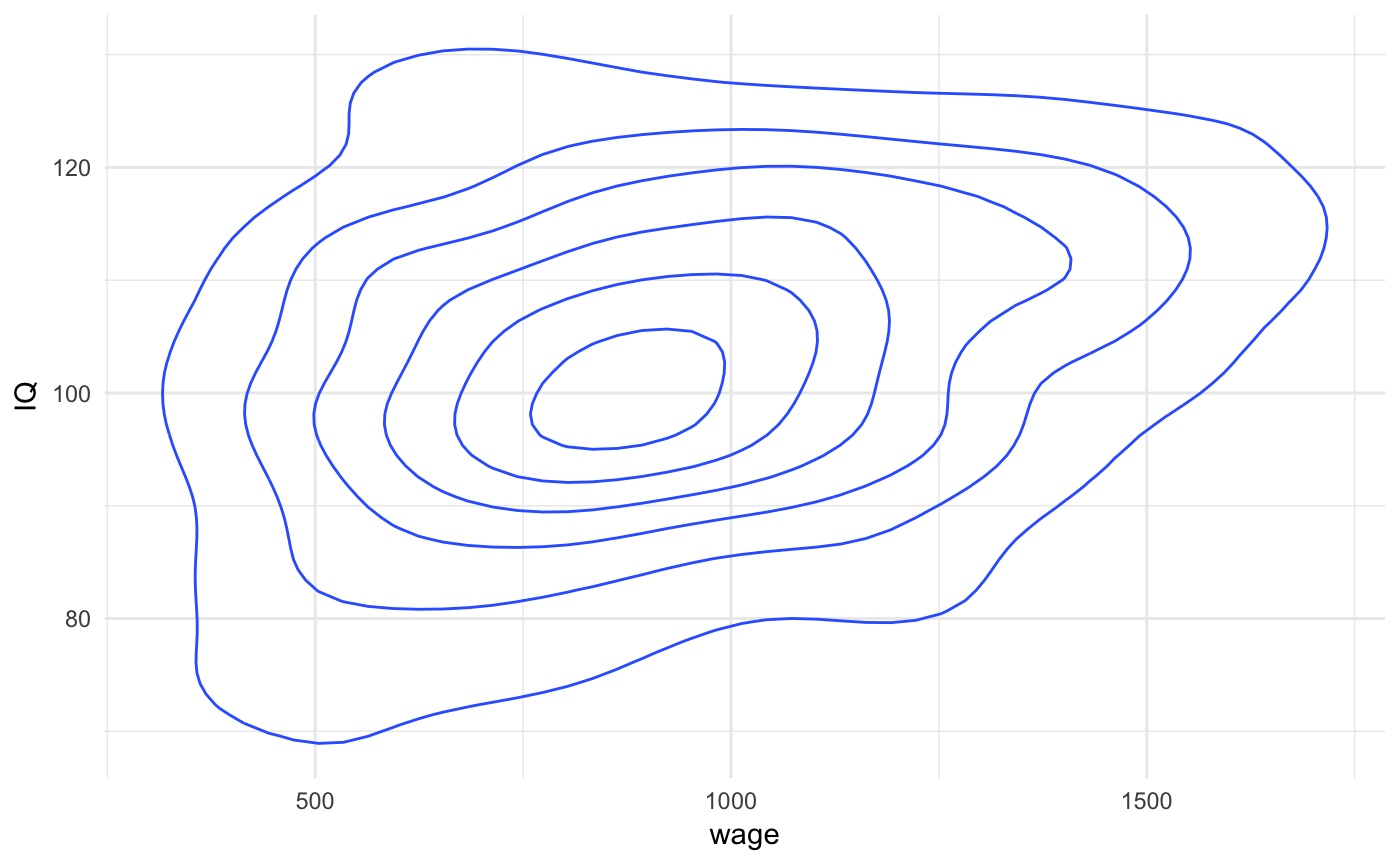
\includegraphics[scale=.25]{PS6a_Hoehne.png}\\
\caption{PS6a | wages2 | density plot of wages and IQ showing distribution of data }
\end{figure}

\begin{figure}
\centering
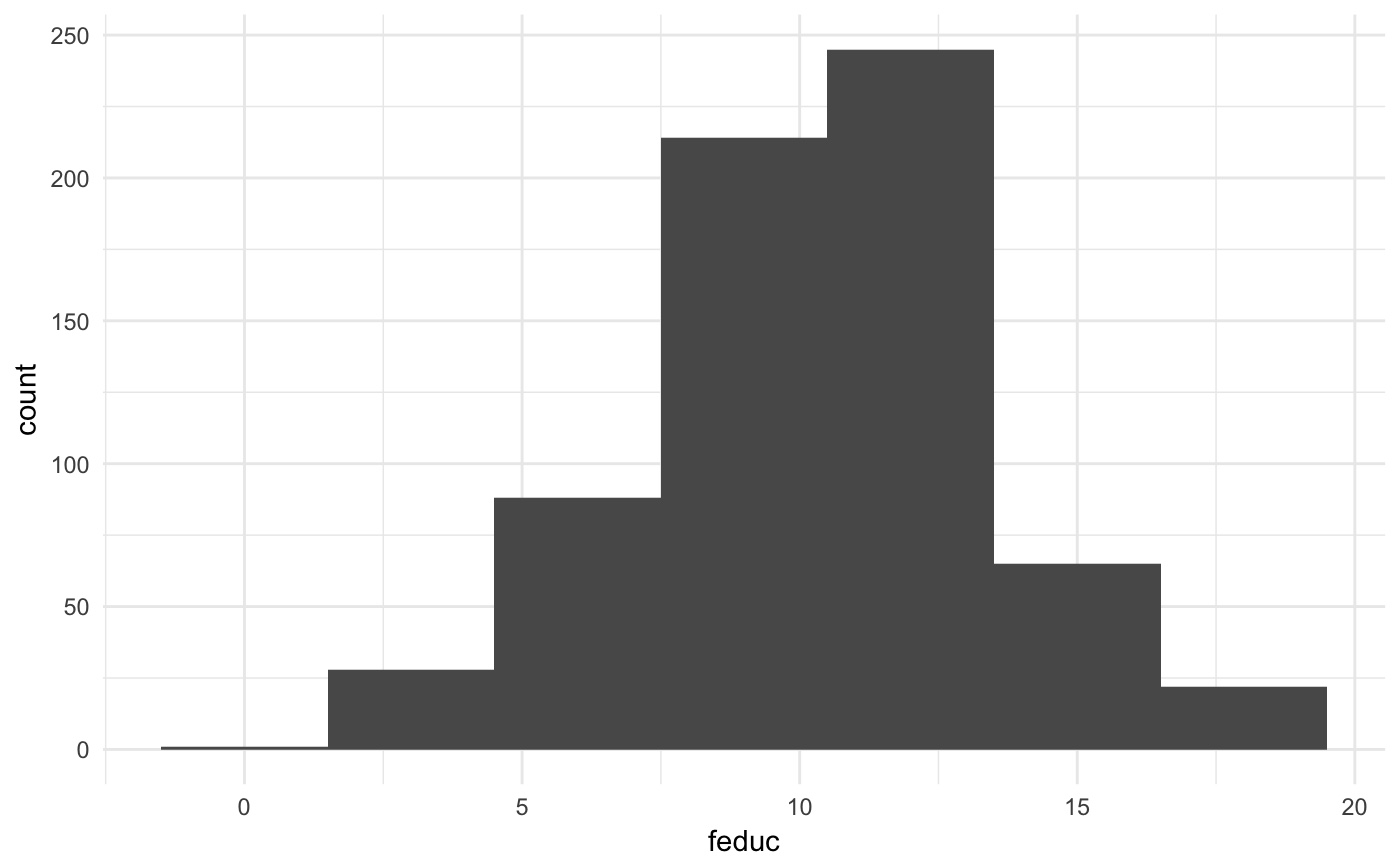
\includegraphics[scale=.25]{PS6b_Hoehne.png}\\
\caption{PS6b | wages2 | histogram of female education in the data set, bins=7 }
\end{figure}

\begin{figure}
\centering
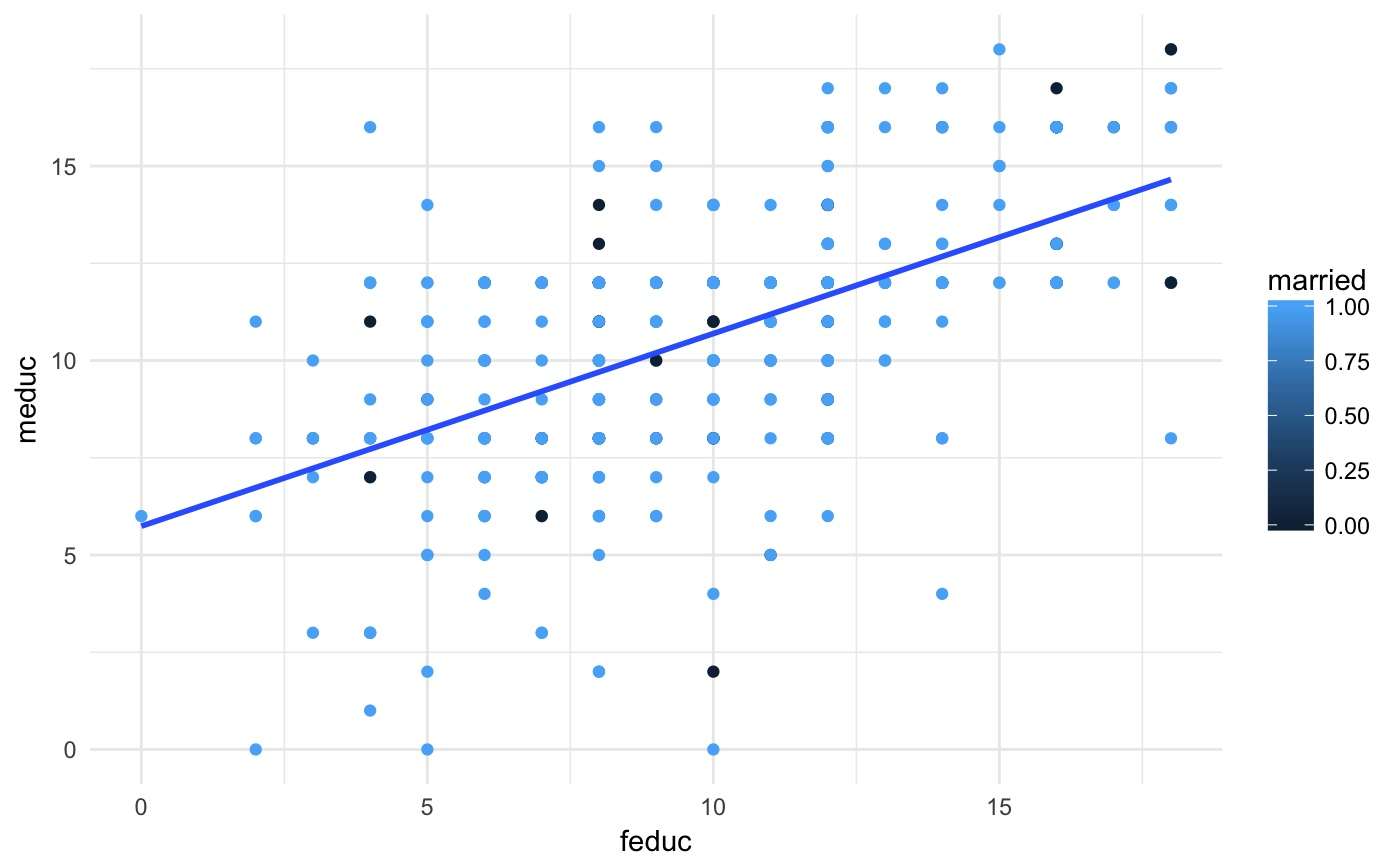
\includegraphics[scale=.25]{PS6c_Hoehne.png}\\
\caption{PS6c | wages2 | simple linear regression on male and female education showing marriage as an indicator}
\end{figure}

\begin{figure}
\centering
\includegraphics[scale=.5]{PS6/P6d_Hoehne.png}\\
\caption{PS6d | iris | plot of different species given their sepal.width and sepal.length with a smoothed trend line, the grey region indicates confidence interval of 95\%}
\end{figure}

\begin{figure}
\centering
\includegraphics[scale=.5]{PS6/P6e_Hoehne.jpg}\\
\caption{PS6e | iris | similar to the above graph without the confidence interval to have a lighter, yet less informative visualization of data}
\end{figure}

\begin{figure}
\centering
\includegraphics[scale=.5]{PS6/P6f_Hoehne.png}\\
\caption{PS6f | iris | linear regression of each species given their sepal.length and sepal.width}
\end{figure}

\begin{figure}
\centering
\includegraphics[scale=.75]{PS6/P6g_Hoehne.jpg}\\
\caption{PS6g | iris | colored histogram of sepal.length indicating each species has a unique and combined range of observations, bins = 30}
\end{figure}

\begin{figure}
\centering
\includegraphics[scale=.5]{PS6/P6h_Hoehne.jpg}\\
\caption{PS6h | iris | density plot showing make up of sepal.length for each species}
\end{figure}

\begin{figure}
\centering
\includegraphics[scale=.5]{PS6/P6i_Hoehne.png}\\
\caption{PS6i | iris | geometric density plot showing locations of each species petal.width and petal.length, notice that the species setosa is an identifiable cluster and that the species versicolor and virginica have an overlapping region}
\end{figure}

\centering

\end{document}
